\documentclass[twocolumn]{revtex4}


% Include some extra packages.
\usepackage[]{graphicx}

\begin{document}

%%%%%%%%%%%%%%%%%%%%%%%%%%%%%%%%%%%%%%%%%%%%%%%%%%%%%%%%%%%%%%%%%%%%%%%%%%%%%%%%
\title{
Monte Carlo Methods
}

\author{Camila Davila}

\affiliation{Siena College, Loudonville, NY}

\date{\today}

\begin{abstract}
 There is a 20\%  chance that it will rain any given day in a month, the odds of it raining one and only one day in a month is 0.9\%. There is also a 10\% chance that it will rain any given day in a month, but the odds of it raining eight days in a month is 0.8\%. The odds of a certain rainfall are as follows: 
 \begin{itemize}
 \item 1 cm 20\% 
 \item 2 cm 30\% 
 \item 3 cm 30\%
 \item 4 cm 10\%
 \item 5 cm 10\%
 
 \end{itemize}
 
 However, the odds of it raining are dependent of the day before. For this particular experiment there will be four scenarios. 
 \begin{enumerate}
 \item First scenario:
 	\begin{itemize}
	\item If it is the first day of the month, there is a 10\% chance of rain.
	\end{itemize}
 
 \item Second scenario:
 	\begin{itemize}
	\item If it rained 1 day before, but not 2 days before, there is a 20\% chance of rain. 
	\end{itemize}

  
  \item Third scenario:
 	\begin{itemize}
	\item If it rained both of the 2 days before, but not the 3rd day before, there is a 25\% chance of rain.
	\end{itemize}
  
  
   \item Fourth scenario:
 	\begin{itemize}
	\item If it rained for the 3 days (or more) before, there is a 5\% chance of rain. 
	\end{itemize}
  
  
 \end{enumerate}
 
 Otherwise, if it does not fit with any of these conditions then there is only a 10\% chance it might rain. 
 We have to find the odds of accumulating at least 10 centimeters of rain in a given month. 
 
 When we have found these values, we have to create a histograms to represent the data.
 
    \end{abstract}

\maketitle
%%%%%%%%%%%%%%%%%%%%%%%%%%%%%%%%%%%%%%%%%%%%%%%%%%%%%%%%%%%%%%%%%%%%%%%%%%%%%%%%

%%%%%%%%%%%%%%%%%%%%%%%%%%%%%%%%%%%%%%%%%%%%%%%%%%%%%%%%%%%%%%%%%%%%%%%%%%%%%%%%
\section{Introduction}

The goal of this project is to predict the weather pertaining to rain fall using Monte Carlo Methods. The Monte Carlo methods are computational algorithms that rely on looped random samples to obtain a numerical value. The essence of this method is using  random number to solve problems. These methods are usually used in Physics and Mathematics to solve problems that are difficult or impossible to use other approaches. Monte Carlo methods are used in every weather report. 
%%%%%%%%%%%%%%%%%%%%%%%%%%%%%%%%%%%%%%%%%%%%%%%%%%%%%%%%%%%%%%%%%%%%%%%%%%%%%%%%


%%%%%%%%%%%%%%%%%%%%%%%%%%%%%%%%%%%%%%%%%%%%%%%%%%%%%%%%%%%%%%%%%%%%%%%%%%%%%%%%
\section{What is the Monte Carlo simulation?}

The Monte Carlo simulation is a computerized technique that allows people to account for risk when making a decision or solving a problem. This method is used by professionals in every field. The variation is so wide, it goes from finance to engineering to the environment. 


This technique was first introduced in World War when some scientists were working on the atomic bomb. The Monte Carlo stimulation has been used to model a variety of physical and conceptual systems. 

\section{How does the Monte Carlo Simulation Works}
This simulation performs risk analysis of possible results by a  "probability distribution", for any factor that experiences uncertainty. It then loops over the calculated result over and over again using a range of random numbers every time from the probability distribution. 

\section{Uses of Monte Carlo}
The most famous use of this method is during the making of the atomic bomb, however today we use it very often. We use it for the analysis of traffic flow on highways, the development of models for the evolution of stars, attempts to predict fluctuations in the stock market and to predict the probability of the weather. 
 \section{Why is the Monte Carlo method so important today}
 
 It is easy and efficient; it tends to be simple, flexible, and scalable. It has its randomness as a strength; it is great for deterministic numerical determination and it simulates a real-life random system. Although it is random there is great insight into its randomness; it has great didactic for exploring and understanding the behavior of the randomness in the systems. Last but not least its theoretical justification; the vast of mathematical and statistical allows for precise and efficient statements. 
 
 
 \section{Monte Carlo in Civil Engineering}
 
 Structural design is done via a deterministic approach. Even if the deterministic designs guarantee some sort of structural safety it is also in our interest to consider the probabilistic approach in order to quantify the safety and reliability that cannot be found in the deterministic design. The deterministic approach is the most widely used by civil engineers when designing structures. 
 \subsection{The Probabilistic Approach}
 Allows engineers to quantify the reliability of the designed structures, as opposed to deterministic design which only allows to determine whether yes or no the structure is safe. The probabilistic designs gives results closer to reality however less conservative than the deterministic design. This method might allow to design structures differently and save on materials and money. 


\subsection{Monte Carlo}

In a probabilistic we model the uncertainty linked to the input parameter such as the applied loads, geometric properties and material properties. Monte Carlo is used to calculate the risk of cost of a design. 


\section{Cost Risk}


In Fig~\ref{ce} we can see how Monte Carlo is used to calculate the probability for the cost not to overrun the estimate. 


\begin{figure}[h]
\center{

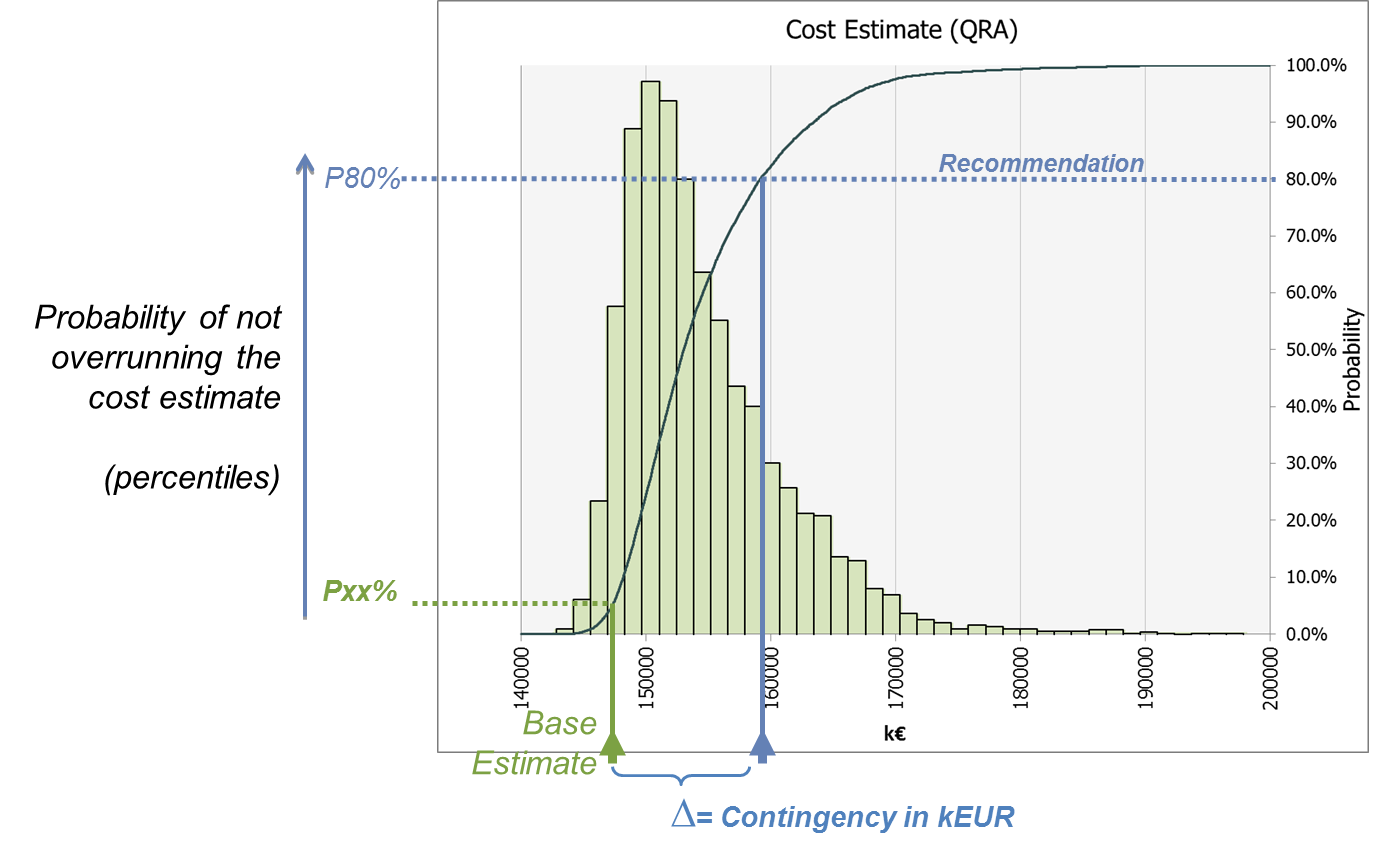
\includegraphics[width = 1\textwidth]{Civil_engineering.png}
\caption{This is a histogram measuring cost risks using Monte Carlo method\label{ce}}}
\end{figure}

%%%%%%%%%%%%%%%%%%%%%%%%%%%%%%%%%%%%%%%%%%%%%%%%%%%%%%%%%%%%%%%%%%%%%%%%%%%%%%%%

%%%%%%%%%%%%%%%%%%%%%%%%%%%%%%%%%%%%%%%%%%%%%%%%%%%%%%%%%%%%%%%%%%%%%%%%%%%%%%%%
\end{document}


%%%%%%%%%%%%%%%%%%%%%%%%%%%%%%%%%%%%%%%%%%%%%%%%%%%%%%%%%%%%%%%%%%%%%%%%%%%%%%%%
